%%==================================================
%% chapter02.tex for TJU Master Thesis
%% based on CASthesis
%% modified by wei.jianwen@gmail.com
%% Encoding: UTF-8
%%==================================================

\chapter{软管组件概述}
\section{引~言}
软管组件经过了几十年的发展演进,经过了大量的研究和实践,已经形成了一系列设计使用的规范。本文第一章已经对软管组件的行业发展进行了简要的介绍,本章着重介绍软管组件的结构,以及加强层理论发展。

\section{软管组件结构}
软管组件,承压能力相对较强,远超普通胶管;结构如图\ref{fig:hose structure}所示,
由内管、加强层、金属连接件组成。根据不同的使用环境一般还有不同种类的的保护层。



\begin{figure}[!htbp]
	\centering
	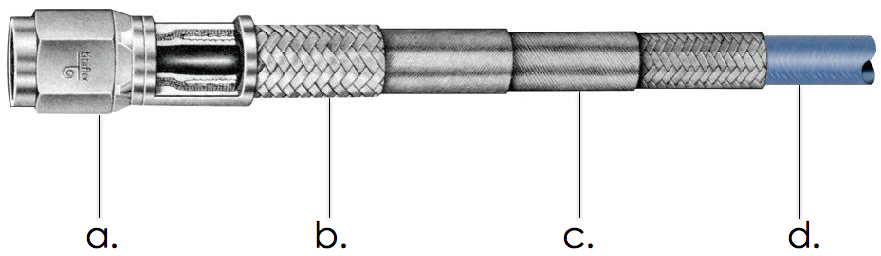
\includegraphics[width=0.6\linewidth]{figure/chap1/Hose-Structure}
	\fcaption{软管组件结构(a.接头,b.金属纤维编织层,c.金属纤维缠绕层,d.内管)}{Hose Structure(a.Coupling,b.Braid Layer,c.Helix-wound Layer,d.Inner Tube)}[软管组件结构]
	\label{fig:hose structure-1}
\end{figure}

\begin{figure}[!htbp]
	\centering
	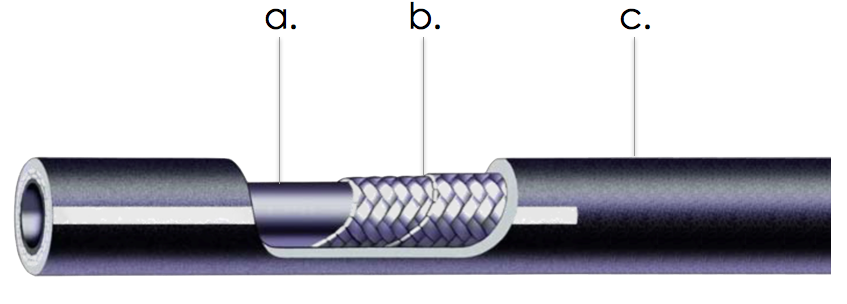
\includegraphics[width=0.6\linewidth]{figure/chap1/Parker-hose}
	\fcaption{软管组件结构(a.内管,b.金属纤维编织层,c.保护套)}{Hose Structure(a.Inner Tube ,b.Braid Layer,c.Coat Tube)}[软管组件结构]
	\label{fig:hose structure-2}
\end{figure}

\subsection{内管}


内管主要起到传输介质的作用,内管直接与油液接触,故要求在长期工作状态下不应受流体腐蚀,能防漏。主要选用的材质是塑料或者橡胶,例如:
\begin{inparaenum}
	\item 
	丁腈橡胶
	\item 
	氯丁橡胶
	\item 
	聚四氟乙烯等。
\end{inparaenum}		
其中,聚四氟乙烯又有“塑料王”之称,它重量轻、耐老化、耐热耐寒性好、抗腐蚀及化学稳定性好,在$ - 60 $\textcelsius \textasciitilde $ +250 $\textcelsius 温度下,可在一定半径范围内随意弯曲,耐疲劳性好,有较大的强度。所以,目前航空界已普遍将它代替传统橡胶内管。传统橡胶内管主要在汽车行业以及大型工程机械中使用。
	
影响性能的主要因素还有内胶层的硬度、厚度和永久变形量。
硬度和永久变形量对密封性能影响很大。
一般硬度高、压缩后的永久变形量小,密封性能则愈好。
一般是在70\textasciitilde 85邵氏硬度,压缩永久变形50\%时为最好。
内胶层厚度最好为1.5\textasciitilde 2.5mm,
厚会在扣压时增加其流动量,造成多余的胶在接头芯套与胶管的接触端面内堆积,减小流通截面;太薄会在扣压时被压裂。
同时内胶层壁厚均匀性也很重要。如果厚度不均,压缩后会造成一面裂断、一面堆胶。
内管表面出现的麻坑也是影响性能质量的重要因素。
	
	
内管成形也是生产软管组件的第一个步骤。以四氟塑料为例,采用的是推挤成形,设备如图\ref{fig:inner-tube-produce}所示。由进料口将粉状的聚四氟乙烯原料通过推挤设备,混料、压坯、推挤、烧结。设备经过合理整合后,控制推挤与烧结速度的配合,可以生产出光滑、均匀的内管,也可以实现大长度连续地生产。











\begin{figure}[!htbp]
	\centering
	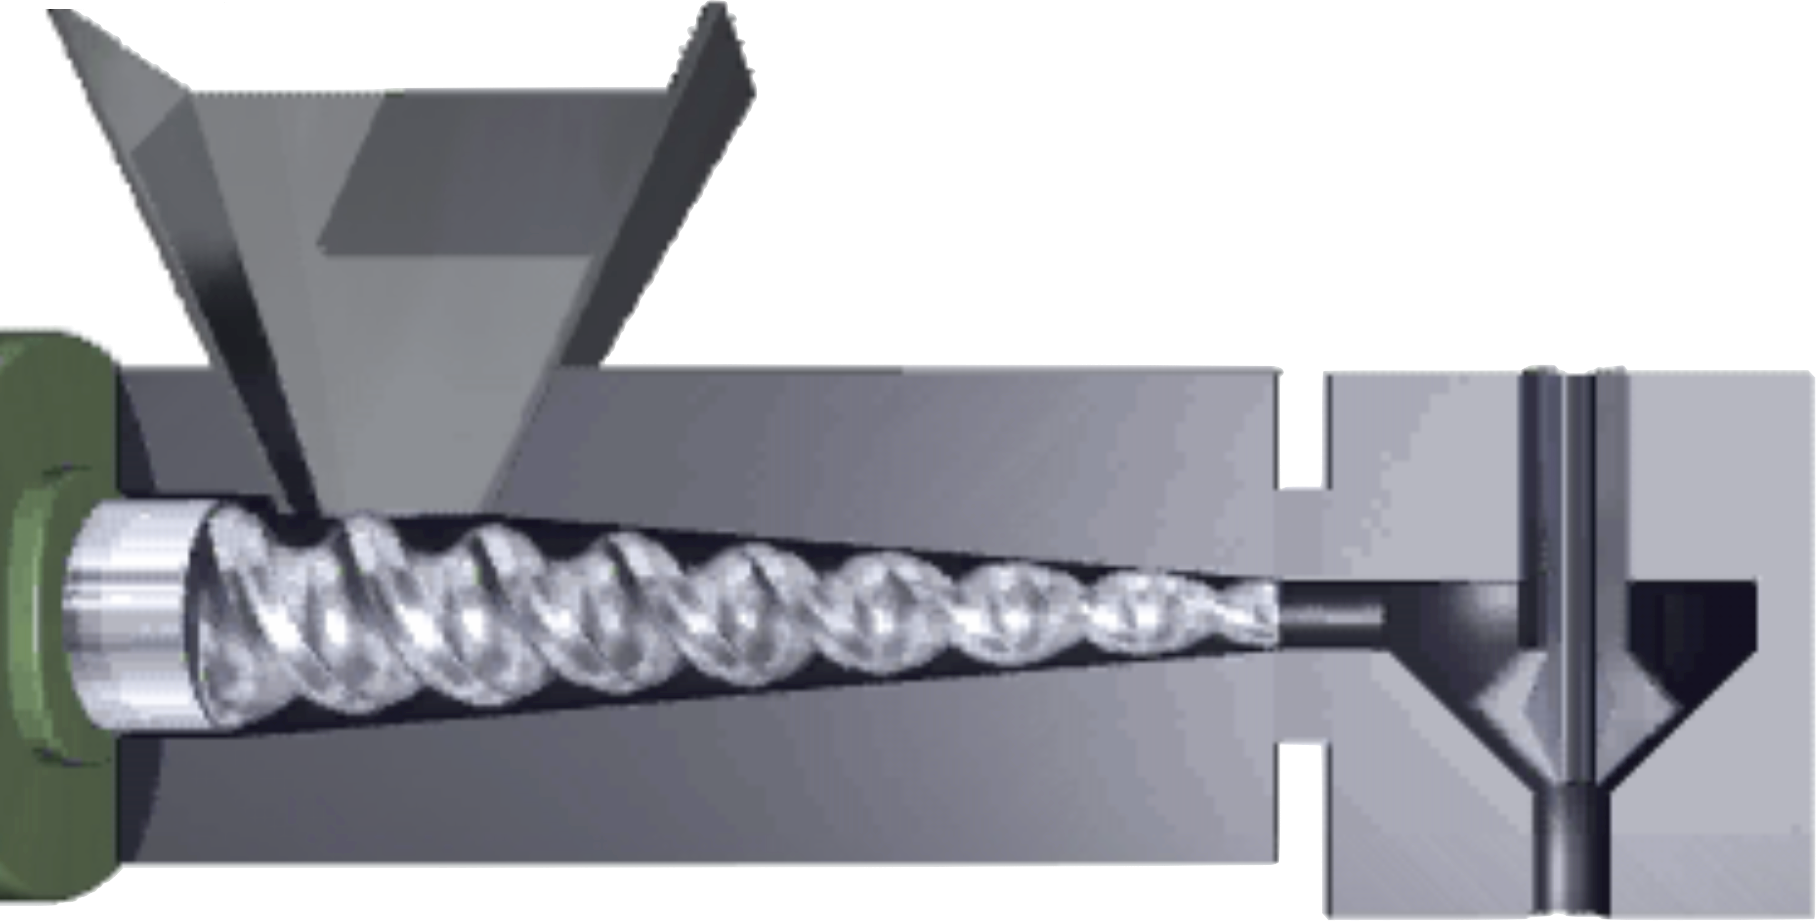
\includegraphics[width=0.4\linewidth]{figure/chap3/Hose/innertube-product}
	\fcaption{内管推挤成形}{inner tube}
	\label{fig:inner-tube-produce}
\end{figure}




\subsection{加强层}

内管成形冷却后就可以进入编织机或者缠绕机,为内管覆盖加强层。

编织机是生产软管组件的重要设备,如图\ref{fig:braider}所示。
编织机主要结构就是一个环形轨道,轨道上安装有两组锭子(spindle),
锭子由洪恩齿轮(Horn Gear)驱动,两组分别沿顺时针和逆时针方向,在圆周轨道上以类似三角函数图像的轨迹运动。
锭子携带若干根一股的金属纤维,使其相互上下交叠形成编织结构。
缠绕机机构与编织机结构相似,只是锭子固定在环形转盘上,随转盘在做圆周运动。

加强层的结构由几个参数控制:
\begin{inparaenum}[1).]
	\item 行程
	\item 编织角
	\item 编织层数。
\end{inparaenum}
这些参数是设计加强层的重中之重,具体在\ref{sec:parameter}节中讨论。

%编织机器图
\begin{figure}[!htbp]
	\centering
	\subfigure[]{
		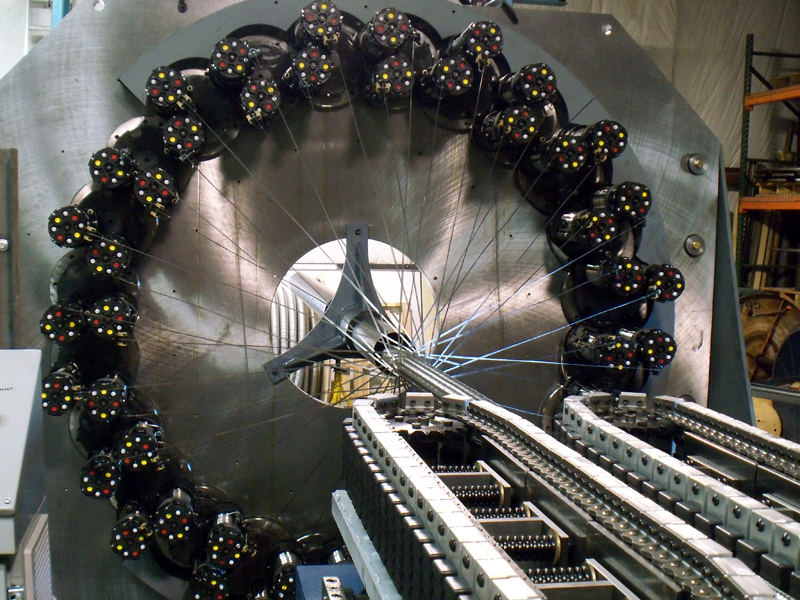
\includegraphics[width=0.4\linewidth]{figure/chap3/Hose/braider-1}}
	\hspace{1cm}
	\subfigure[]{
		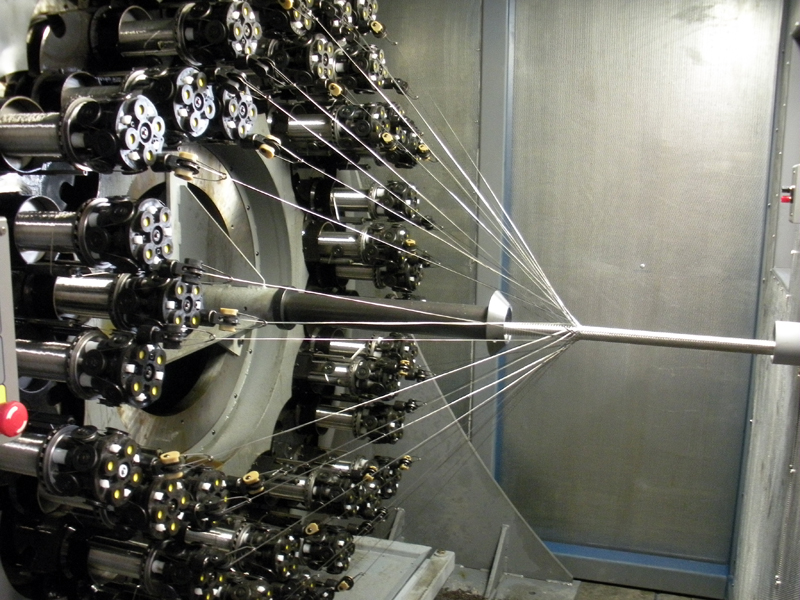
\includegraphics[width=0.4\linewidth]{figure/chap3/Hose/braider-2}}
	\subfigure[]{
		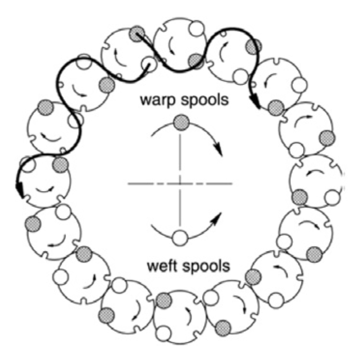
\includegraphics[width=0.3\linewidth]{figure/chap3/Hose/braider-theory}\label{fig:braider-theory-a}}
	\hspace{1cm}
	\subfigure[]{
		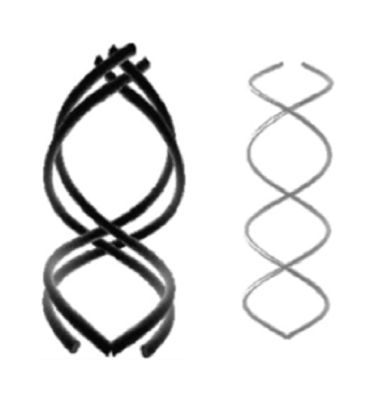
\includegraphics[width=0.3\linewidth]{figure/chap3/Hose/braider-theory-2}\label{fig:braider-theory-b}}
	\fcaption{编织机原理}{Braider}
	\label{fig:braider}
\end{figure}	

加强层是软管组价主要的承力结构,主要有编织和缠绕两种加强形式。对比两种加强层形式,各有优缺点。

缠绕层一般成对出现。所谓“成对”是指,缠绕加强时,不能只沿顺时针或逆时针方向缠绕,而必须反向的两层一组,来保持结构的受力平衡。
缠绕层中,金属纤维贴靠更为紧密,因而可以耐受更高的内压荷载,同时与内管贴合更好,不容易损伤内管。
另外缠绕层中的金属纤维弯曲半径较大,相互之间的接触关系较也相对比较简单,在两层之间有一般有中间胶,因此同一工作层的两层金属纤维之间没有交叉点。因而在承受动压时,不会因为金属纤维的交叉弯曲而产生应力集中或摩擦磨损。因此寿命要长于编织层,高频振动的环境优先选择缠绕加强。




但是缠绕层并不是一个稳定的结构,必须配合编织层,或者紧密贴合的橡胶套管,如\ref{fig:helix-tube-example}所示。因此缠绕加强一般比较笨重,多用于重型软管组件。


\begin{figure}[!htbp]
	\centering
	\subfigure[]{
		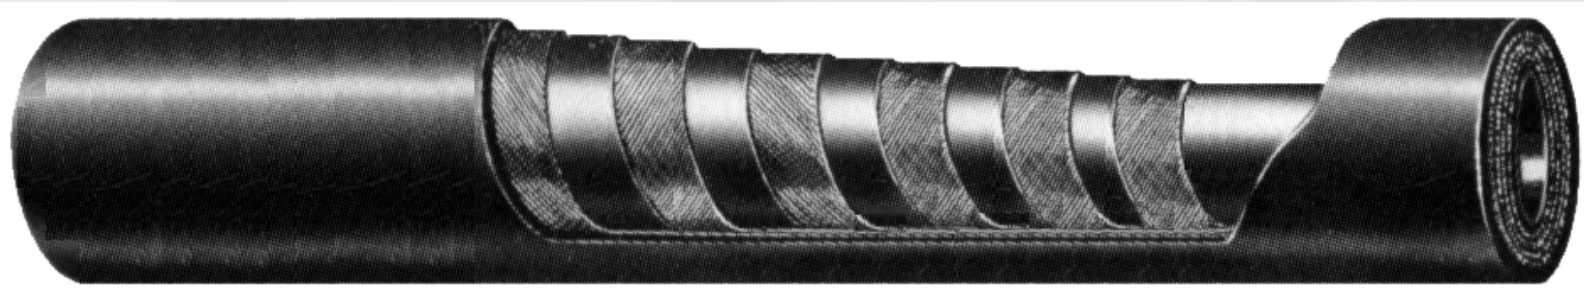
\includegraphics[width=0.45\linewidth]{figure/chap3/Hose/helix}\label{fig:helix-tube-example}}
	\hspace{1cm}
	\subfigure[]{
		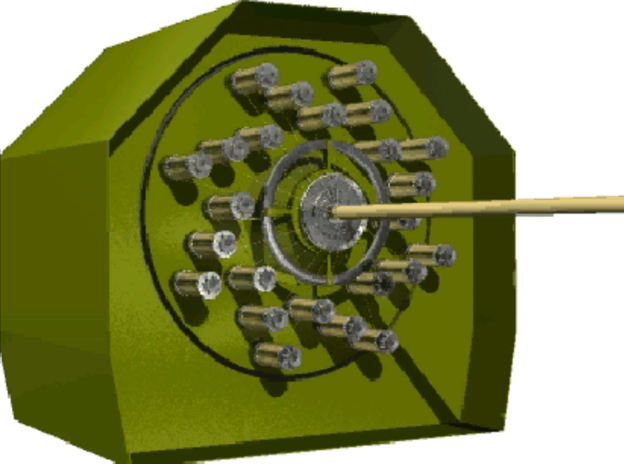
\includegraphics[width=0.3\linewidth]{figure/chap3/Hose/helix-wounder}\label{fig:helix-wounder}}
	\fcaption{占位图}{place holder}
	\label{fig:helix-tube}
\end{figure}


编织层中,纤维穿插交织形成了一个稳定的结构。一层编织相当于两层缠绕。由于同一编织层内钢丝之间的相互接触,在承受动压时,会因各自伸缩不一而造成钢丝相互之间的磨擦而影响其耐久性。
但是编织层自身就能形成稳定的加强结构,不需要其他结构辅助,非常轻巧。因此在轻型高压的软管组件中,必须使用编织层。



	
	
\subsection{金属连接件}
	\begin{asparaenum}
		\item 扣压式\\
		依靠接头公装的塑性变形和摩擦力形成有效连接。
		\item 分离式\\
		编织层覆盖系数小于缠绕曾,结构稳定,弯曲性能稳定,不会松散。
		
		\ref{fig:placeholder}
		\ref{fig:placeholder:a}
		\begin{figure}[!htbp]
			\centering
			\subfigure[]{\label{fig:placeholder:a}
				
\includegraphics[width=0.4\linewidth]{figure/placeholder}}
			\hspace{1cm}
			\subfigure[]{
				
\includegraphics[width=0.4\linewidth]{figure/placeholder}}
			\fcaption{占位图}{placeHolder}
			\label{fig:placeholder}
		\end{figure}
	\end{asparaenum}	
	





	




\section{软管组件加强层参数}
\label{sec:parameter}



\subsection{编织角}


\subsection{编织密度}


\subsection{编织层数}






\section{软管组件性能参数}

软管组件主要包括一下几个重要的参数:
\begin{compactenum}
	\item 最大工作压力\\
	胶管在使用时所能承受的最大压力包括瞬间的峰值压力
	\item 试验压力\\
	软管耐压试验使用的压力,通常是额定压力的2倍
	\item 最小爆破压力\\
	使胶管破裂时所使用的真实压力,最小爆破压力通常是额定压力 的4倍
	\item 弯曲半径\\
	在不影响软管寿命的情况下软管所能弯曲的半径
	\item 长度变化\\
\end{compactenum}




\section{软管组件验证实验}
为了保证软管组件安全工作,美国、欧洲和国际标准都规定了一下几个重要的实验:
\begin{compactenum}
	\item 爆破实验\\
	以一定的升压速率,增加内压,直到软管组件发生渗漏、接头发生脱头或者管体破裂。以此时的压力值为软管组价的最小爆破压力。
	
	\begin{figure}[!htbp]
		\centering
		\subfigure[]{
			
\includegraphics[width=0.4\linewidth]{figure/placeholder}}
		\subfigure[]{
			
\includegraphics[width=0.4\linewidth]{figure/placeholder}}
		\fcaption{占位图}{place holder}
		\label{fig:placeholder}
	\end{figure}
	
	\item 试验压力\\
	软管耐压试验使用的压力,通常是额定压力的2倍
	\item 脉冲实验\\
	按照规定压力、频率施加脉冲荷载,反复施加直到管体破坏。
\end{compactenum}	



